\documentclass[10pt]{report}
\usepackage{graphicx,color,epsfig,psfig,subfigure}
\usepackage{amsmath,amsfonts,amssymb}
\usepackage{bm}
\pagestyle{empty}
\begin{document} 
\begin{picture}(0,0)%
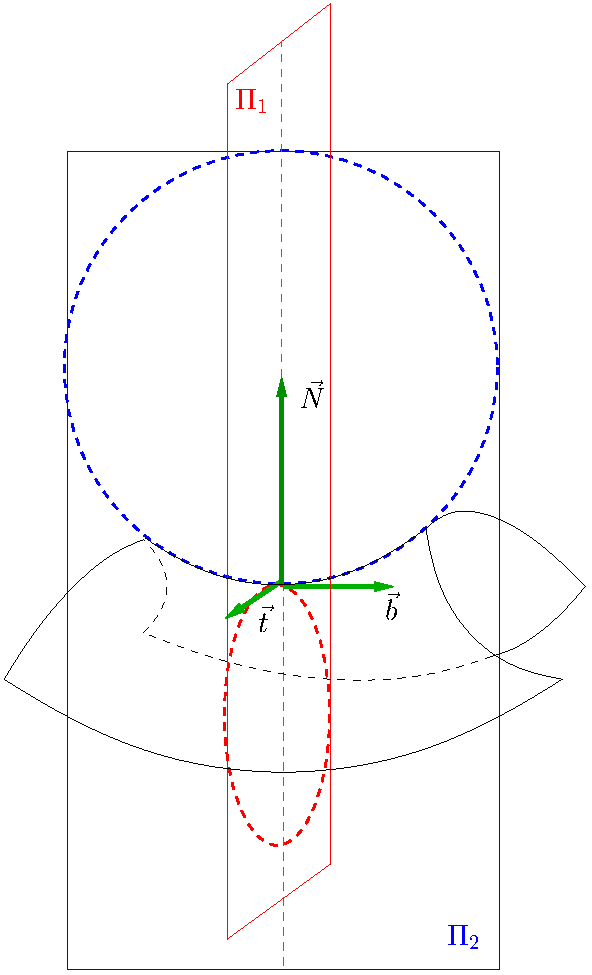
\includegraphics{courbure_surface.pstex}%
\end{picture}%
\setlength{\unitlength}{3947sp}%
%
\begingroup\makeatletter\ifx\SetFigFont\undefined%
\gdef\SetFigFont#1#2#3#4#5{%
  \reset@font\fontsize{#1}{#2pt}%
  \fontfamily{#3}\fontseries{#4}\fontshape{#5}%
  \selectfont}%
\fi\endgroup%
\begin{picture}(4674,7749)(6094,-8113)
\put(8476,-3600){\makebox(0,0)[lb]{\smash{\SetFigFont{14}{16.8}{\familydefault}{\mddefault}{\updefault}{\color[rgb]{0,0,0}$\vec{N}$}%
}}}
\put(9166,-5296){\makebox(0,0)[lb]{\smash{\SetFigFont{14}{16.8}{\familydefault}{\mddefault}{\updefault}{\color[rgb]{0,0,0}$\vec{b}$}%
}}}
\put(8146,-5386){\makebox(0,0)[lb]{\smash{\SetFigFont{14}{16.8}{\familydefault}{\mddefault}{\updefault}{\color[rgb]{0,0,0}$\vec{t}$}%
}}}
\put(9661,-7891){\makebox(0,0)[lb]{\smash{\SetFigFont{14}{16.8}{\familydefault}{\mddefault}{\updefault}{\color[rgb]{0,0,1}$\Pi_2$}%
}}}
\put(7966,-1201){\makebox(0,0)[lb]{\smash{\SetFigFont{14}{16.8}{\familydefault}{\mddefault}{\updefault}{\color[rgb]{1,0,0}$\Pi_1$}%
}}}
\end{picture}
\end{document}
